\chapter{State of the art} \label{state_of_the_art}

In this chapter is of the utmost importance to define some concepts that were used has a basis for this thesis. In addition, it will be discussed possible tools that already answer some of the questions that this thesis is trying to answer, and for that matter are important to be studied and referenced.
	
\section{Domain Specific Language}
A domain specific language is an ``executable specification language, through appropriate notations and abstractions'', usually restricted to a particular problem domain. Their objective is to improve productivity, and to allow solutions to be expressed in the idiom and at the level of abstraction of the problem domain \cite{van_2000}.
	
This types of languages provide a natural vocabulary for concepts that are fundamental to the problem scope \cite{bruce_1997}, something that may lack when using a general-purpose language. \textsc{DSLs} are usually small and declarative, with very specific goals \cite{van_2000}. Refered as ``little languages'' \cite{bentley_1986}, they are intended to solve problems within a specific domain, and not outside it.
	
\section{Attribute Grammar}
Attribute Grammars were proposed by Donald Knuth in order to specify static and dynamic semantics of a programming language in a syntax-directed manner \cite{thirunarayan_2009}. The process consists in constructing the syntax tree and then computing the values of attributes by visiting every single node. For each attribute it is possible to associate a domain of values, such as integers, strings or even complex structures. Formally an attribute grammar (AG) is a tuple \cite{pereira_2016}

AG = \textless CFG, A, CR, CC, TR\textgreater

\noindent that is composed by a context-free grammar (CFG), which has been extended to provide context by using a set of attributes; Those same set of attributes (A), which exist in each production of a grammar, and are divided into two groups, \emph{Synthezized Attributes}, which allows values to be pass one from a node to its parent, and \emph{Inherited Attributes}, which allows values to be pass on from the current node to a child \cite{slonneger_1995}; rules for calculating attributes (CR) in all productions of the grammar; a set of contextual conditions (CC); and the transformation rules (TR) in all productions of the grammar.

\section{PAG (Prototyping with Attribute Grammars)}
PAG is a tool that was created with the purpose of helping two distinct groups of students from \emph{Universidad Complutense de Madrid}. One of those groups, involving computer science students, that attended a class which teached compiler contructions, and other group involving linguistic students, with a class on computacional linguistics. Teachers from both classes used the same methodology to teach their classes, na dnoticed that it wasnt good enough for the students to master all the concepts: On one hand, they would have computer science skilled students, with great apititude to produce solutions, but leaving aside the respective specifications, which lead to poor and innacurate formal specifications, but on the other hand, linguistic students produced good formal specifications, as they are proficient with the natural language, but lack computer science skills to well transpose all the knowledge into computacional models \cite{sierra_2006}.
	
The result was an environment based in attribute grammars that allows the specification of those same grammars using a language close to Prolog. The main goal was to embed Prolog into the language and maintain all the familiar basic notation, the reason being both groups of students were already familiar with the Prolog and attribute grammar syntax and notation. Through rapid prototyping, which PAG makes use of, it is possible to obtain a functional processor at a embryonic state of the problem \cite{sierra_2006}. With this, computer science students can obtain results quite early, allowing them to apply more time into formal specifications. Moreoever, as the complexity of the syntax is reduced, this allows for a better and easier learning experience for students which have less aptitude for the solution codification or programming in general, which is the case for linguistic students.
	
Overall, PAG solved the problem that was purposed in an effective way. Despite that, and giving the respective credit to the those who built the tool, the fact is that Prolog can still be quite difficult to grasp for some people, and a challenge when it comes to learn it. The usage of a specification language that closely resembles the natural one, could be a great addition.
	
\section{VisualLISA (A Visual Programming Environment for Attribute Grammars)}
VisualLISA is a visual programming environment created by Pedro Oliveira in the year of 2009 \cite{oliveira_2009} for the specification of attribute grammars. Classified as a ``Domain Specific  Visual Language'', its main goal was to enhance the front-end of one other tool named LISA \footnote{https://labraj.feri.um.si/lisa/}, a compiler generator based in AG's that creates different visual tools based on the textual specification of the grammars.
    
The aim of this tool was to decrease the difficulty which is involved with specifying attribute grammars, not only for the LISA environment, but also regarding other types of systems, making specifications more visual and graphical.
    
Specifying grammars in a visual manner can be done using a set of icons (\autoref{fig:visuallisa_icons}) that must be combined to obtain the wanted result. Each icon or symbol has a unique function, and it is the users task to make the connections in a correct way.
    
% Imagem dos icons do VisualLISA
\begin{figure}[h]
    \centering
    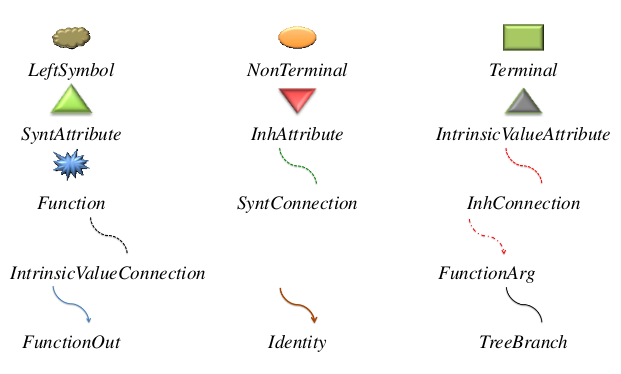
\includegraphics[width=10cm]{images/visuallisa_icons.png}
    \caption{VisualLISA set of icons.}
    \label{fig:visuallisa_icons}
\end{figure}

\newpage
The environment (\autoref{fig:visuallisa_window}) consists in 4 windows, each one with an individual task: declare the productions of the grammar in a textual manner; declare functions, data-types, etc. ; draw the grammar productions; specify computation rules that were previously declared.
    
% Imagem da janela do VisualLISA
\begin{figure}[h]
    \centering
    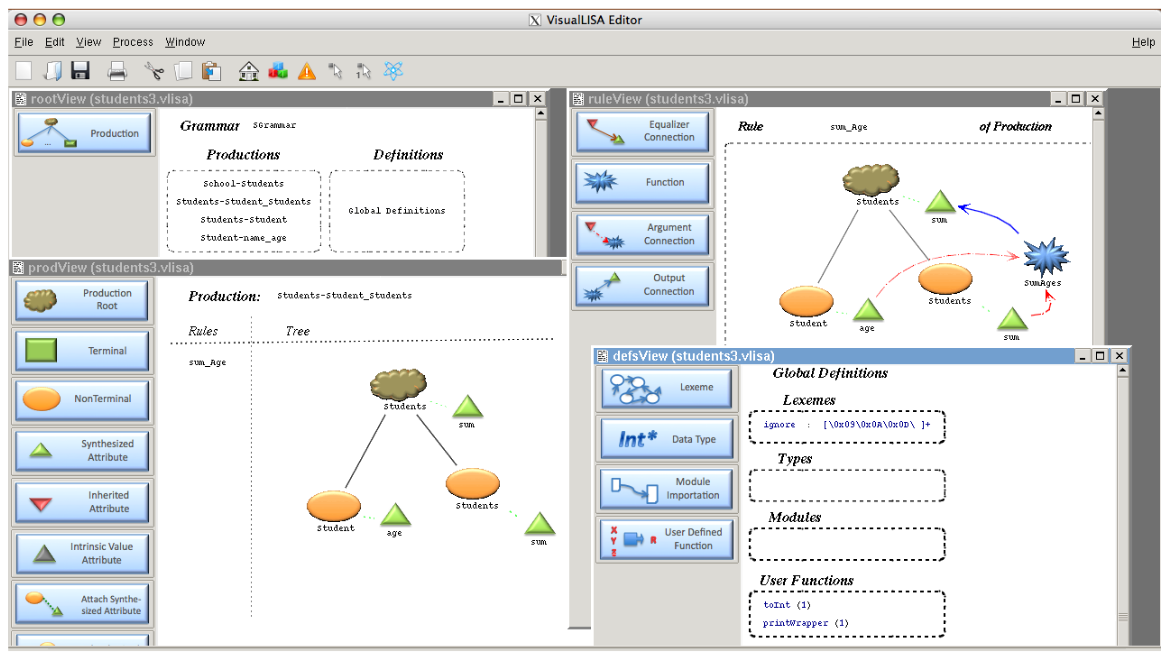
\includegraphics[width=10cm]{images/visuallisa_window.png}
    \caption{VisualLISA main window.}
    \label{fig:visuallisa_window}
\end{figure}
    
As an example, it was included a textual specification (\autoref{fig:textual_students_grammar}) and the respective graphical specification (\autoref{fig:graphical_students_grammar}), extracted from the proper article \cite{oliveira_2009}.
    
% Students Grammar
\begin{figure}[h]
    \centering
    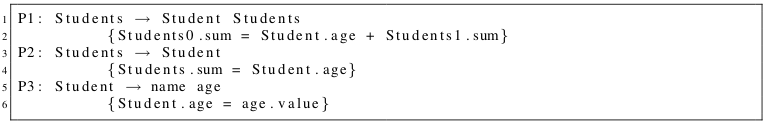
\includegraphics[width=15cm]{images/textual_students_grammar.png}
    \caption{Students textual grammar.}
    \label{fig:textual_students_grammar}
\end{figure}

\newpage

% VisualLISA Conception
\begin{figure}[h]
    \centering
    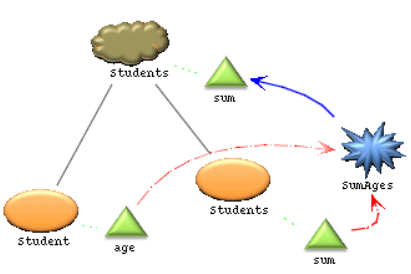
\includegraphics[width=8cm]{images/graphical_students_grammar.png}
    \caption{Students graphical grammar.}
    \label{fig:graphical_students_grammar}
\end{figure}

The main effect of the tool is not directly related to the problem that is trying to be solved, what is useful are all the visual components that are associated with it, which could help when creating the intended user interface for the visual analysis of the generated syntax-tree, or more. Nevertheless, it is a very useful and interesting way of aproaching attribute grammars and their specifications.
